\documentclass[12pt, a4paper, twoside]{article}

\usepackage{tex/style/snowrake}
\usepackage{amsmath, bm, tikz, subfig, nicematrix}
\usetikzlibrary{calc} 

\author{Gábor Szijártó}
\title{Recalling Trigonometric Identities}
\date{}
\renewcommand{\srcompany}{Medium}
\renewcommand{\srtitle}{}
\renewcommand{\srdocver}{v0}
\newcommand{\mat}[1]{\bm{#1}}
%\captionsetup[subfigure]{labelformat=empty}

\begin{document}

\srdocsimple

In this post I'll share an easy way to derive and remember trigonometric identities.\\

Surprisingly, all you need to know:
\begin{itemize}
\item $cos(\varphi) = \frac{hypotenuse}{adjacent side}$
\item matrix multiplication
\end{itemize}

If you can remember the 2D rotation matrix you can jump through this section!\\
It can be easily constructed based on the rotation of the (1, 0) and (0, 1) vectors.

\begin{equation}
	\begin{pmatrix}1, 0\end{pmatrix} \to \begin{pmatrix}C_{\varphi}, S_{\varphi}\end{pmatrix}
	\quad \quad \quad
	\begin{pmatrix}0, 1\end{pmatrix} \to \begin{pmatrix}-S_{\varphi}, C_{\varphi} \end{pmatrix}
\end{equation}

\begin{figure}[H]
	\hfill \subfloat[]{
		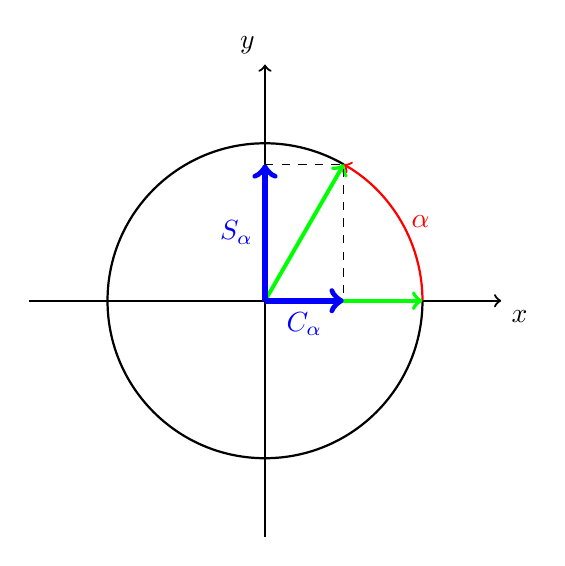
\begin{tikzpicture}[scale=1]
			\def\size{3.0}
			\def\rad{2.0}
			\coordinate (O) at (0,0);
			
			% Draw axes
			\draw[->, thick] (-\size,0) -- (\size,0) node[anchor=north west] {$x$}; % x-axis
			\draw[->, thick] (0,-\size) -- (0,\size) node[anchor=south east] {$y$}; % y-axis
			
			\coordinate (Xr) at ({\rad*cos(60)},0);
			\coordinate (Yr) at (0,{\rad*sin(60)});
			\draw [->, thick, red] (O)++(\rad,0) arc(0:60:\rad) node[midway, anchor=west]{$\alpha$};
			
			\draw[thick] (O)++(\rad,0) arc(0:-300:\rad);
			\draw[->, green, line width=0.5mm] (O) -- (\rad,0);
			\draw[->, green, line width=0.5mm, rotate=-30] (O) -- (0,\rad);
			\draw[->, blue, line width=0.75mm] (O) -- (Xr) node[midway, anchor=north] {$C_\alpha$};
			\draw[->, blue, line width=0.75mm] (O) -- (Yr) node[midway, anchor=east] {$S_\alpha$};
			\draw[-, dashed] (Yr)--($(Xr) + (Yr)$)--(Xr);
		\end{tikzpicture}
	}
	\subfloat[]{
		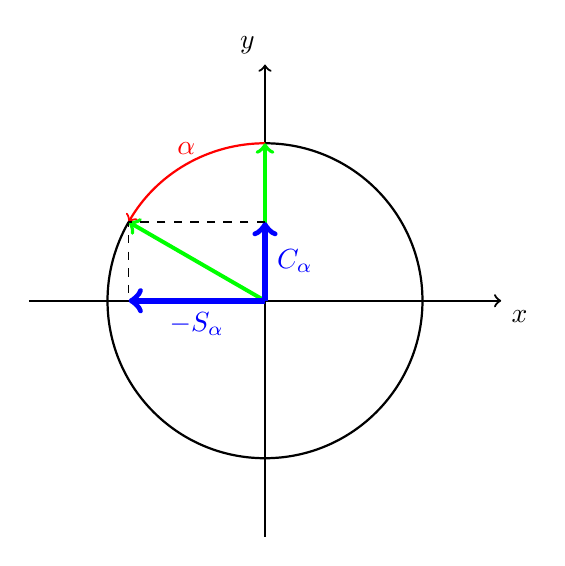
\begin{tikzpicture}[scale=1]
			\def\size{3.0}
			\def\rad{2.0}
			\coordinate (O) at (0,0);
			
			% Draw axes
			\draw[->, thick] (-\size,0) -- (\size,0) node[anchor=north west] {$x$}; % x-axis
			\draw[->, thick] (0,-\size) -- (0,\size) node[anchor=south east] {$y$}; % y-axis
			
			\coordinate (Xr) at ({-1*\rad*sin(60)},0);
			\coordinate (Yr) at (0,{\rad*cos(60)});
			\draw [->, thick, red] (O)++(0,\rad) arc(90:150:\rad) node[midway, anchor=south]{$\alpha$};
			
			\draw[thick] (O)++(0,\rad) arc(90:-210:\rad);
			\draw[->, green, line width=0.5mm] (O) -- (0,\rad);
			\draw[->, green, line width=0.5mm, rotate=60] (O) -- (0,\rad);
			\draw[->, blue, line width=0.75mm] (O) -- (Xr) node[midway, anchor=north] {$-S_\alpha$};
			\draw[->, blue, line width=0.75mm] (O) -- (Yr) node[midway, anchor=west] {$C_\alpha$};
			\draw[-, dashed] (Yr)--($(Xr) + (Yr)$)--(Xr);
	\end{tikzpicture}}
	\hfill
\end{figure}

\begin{equation}
	\mat{rot_{\varphi}}=\begin{pmatrix} C_{\varphi} & -S_{\varphi} \\ S_{\varphi} & C_{\varphi}\end{pmatrix}
\end{equation}
\pagebreak

I won't give proper mathematical background or prove intuitive assumptions like rotating a vector by $\alpha$ and then
by $\beta$ around the same point gives the same result as a single rotation of $\alpha + \beta$. \\

\begin{equation} \begin{aligned}
	\mat{rot_{\alpha + \beta}} &= \mat{rot_{\alpha}} \, \mat{rot_{\beta}}\\[0.5em]
	\begin{pNiceMatrix} \Block[fill=blue!20,rounded-corners]{1-1}{C_{\alpha + \beta}} & -S_{\alpha + \beta} \\ S_{\alpha + \beta} & C_{\alpha + \beta} \end{pNiceMatrix} &=
	\begin{pNiceMatrix} \Block[fill=blue!20,rounded-corners]{1-2}{} C_{\alpha} & -S_{\alpha} \\ S_{\alpha} & C_{\alpha} \end{pNiceMatrix}
	\begin{pNiceMatrix} \Block[fill=blue!20,rounded-corners]{2-1}{} C_{\beta} & -S_{\beta} \\ S_{\beta} & C_{\beta} \end{pNiceMatrix}
\end{aligned} \end{equation}

\begin{equation}
	C_{\alpha + \beta} = C_\alpha C_\beta - S_\alpha S_\beta
\end{equation}

The addition formula for the sine can be calculated by the same way, just using the dot product of the corresponding rows and columns.\\

Have this one in the bag you can easily derive other identities, see the link below.\\

The post was written as an addition to \href{https://blog.keithmcnulty.org/the-two-key-trig-identities-worth-memorizing-3df894d5f216}{'The Two Key Trig Identities Worth Memorizing'}
\end{document}
